\documentclass[aspectratio=169,11pt,t]{beamer}
% Final slides. Figures and result tables are the report's own (figures/, generated/), so the
% numbers cannot drift from it. Build: latexmk -pdf slides.tex
\usetheme{default}
\usepackage[dvipsnames,table]{xcolor}
\usepackage{booktabs,tabularx,array}
\usepackage{tikz}
\usetikzlibrary{arrows.meta,positioning,shapes.geometric,fit,backgrounds}
\usepackage{pgfplots,pgfplotstable}
\pgfplotsset{compat=1.17}
\pgfplotsset{every axis/.append style={font=\small}}

% Palette: the college navy, a muted gold accent, soft paper tints for panels.
\definecolor{bmsblue}{RGB}{0,51,102}
\definecolor{bmsdeep}{RGB}{0,34,72}
\definecolor{bmsgold}{RGB}{201,154,46}
\definecolor{guidebg}{RGB}{235,241,249}
\definecolor{dobg}{RGB}{230,245,233}
\definecolor{dontbg}{RGB}{252,232,232}
\definecolor{inkgray}{RGB}{70,78,92}
\definecolor{rulegray}{RGB}{200,206,216}

\setbeamercolor{structure}{fg=bmsblue}
\setbeamercolor{normal text}{fg=black!85}
\setbeamercolor{title}{fg=white}
\setbeamercolor{block title}{bg=bmsblue,fg=white}
\setbeamercolor{block body}{bg=guidebg,fg=black!85}
\setbeamercolor{block title alerted}{bg=BrickRed!85!black,fg=white}
\setbeamercolor{block body alerted}{bg=dontbg,fg=black!85}
\setbeamerfont{block title}{series=\bfseries,size=\normalsize}
\setbeamertemplate{blocks}[rounded][shadow=false]
\setbeamertemplate{navigation symbols}{}
\setbeamersize{text margin left=1.1cm,text margin right=1.1cm}

% Bullets: small gold squares, navy sub-bullets.
\setbeamertemplate{itemize item}{\raisebox{0.15ex}{\color{bmsgold}\tiny$\blacksquare$}}
\setbeamertemplate{itemize subitem}{\raisebox{0.15ex}{\color{bmsblue}\tiny$\blacktriangleright$}}
\setbeamerfont{itemize/enumerate body}{size=\normalsize}

% Frame title: full-width navy band with a gold rule; the title sits on the band.
\setbeamertemplate{frametitle}{%
  \begin{tikzpicture}[remember picture,overlay]
    \fill[bmsblue] (current page.north west) rectangle ([yshift=-1.0cm]current page.north east);
    \fill[bmsgold] ([yshift=-1.0cm]current page.north west) rectangle ([yshift=-1.07cm]current page.north east);
    \node[anchor=west,text=white,font=\Large\bfseries] at ([xshift=1.1cm,yshift=-0.5cm]current page.north west) {\insertframetitle};
  \end{tikzpicture}\vskip0.4cm}

% Footer: hairline, team on the left, page counter on the right.
\setbeamertemplate{footline}{%
  \leavevmode\hbox to\paperwidth{\hspace*{1.1cm}\vrule width\dimexpr\paperwidth-2.2cm\relax height 0.4pt depth 0pt\hss}\par\nointerlineskip
  \vskip0.15cm
  \hbox to\paperwidth{\hspace*{1.1cm}\color{inkgray}\scriptsize ReCycleGuard \textbullet\ Agentic AI \textbullet\ Team 06\hfill
    \color{bmsblue}\bfseries\insertframenumber\,/\,\inserttotalframenumber\hspace*{1.1cm}}%
  \vskip0.3cm}
\setbeamertemplate{caption}{\raggedright\insertcaption\par}
\setbeamerfont{caption}{size=\scriptsize}

\newsavebox{\fitbox}
\newcommand{\shrinkfit}[1]{\sbox{\fitbox}{#1}%
  \ifdim\wd\fitbox>\linewidth\resizebox{\linewidth}{!}{\usebox{\fitbox}}\else\usebox{\fitbox}\fi}
% The generated tables set \small; on a slide they need to be smaller.
\newcommand{\slidetable}[1]{\begingroup\renewcommand{\small}{\scriptsize}\renewcommand{\caption}[1]{}\renewcommand{\smallskip}{\vspace{0.6em}}\input{#1}\endgroup}
% The held-out slide carries its own commentary, so the generated table's footnote is dropped.
\newcommand{\HeldOutTable}{\IfFileExists{generated/heldout.tex}{\begingroup\renewcommand{\parbox}[2]{}\slidetable{generated/heldout.tex}\endgroup}%
  {\begin{center}\fbox{\parbox{0.8\linewidth}{\centering\textbf{Held-out result pending}: the run
  declared in log entry 15 had not been scored when these slides were built.}}\end{center}}}

\title{ReCycleGuard}
\subtitle{An audited agentic assistant for e-waste EPR reconciliation}
\author{Team 06: H Sampreeth Bhat (1BM23CD020), R V Abhishek (1BM23CD047),\\
Sushanth S (1BM23CD063), Vedantha Vinay Vernekar (1BM23CD069)}
\institute{Agentic AI (26CD7PEAAI), Dept.\ of CSE (Data Science), B.M.S. College of Engineering\\
Course lead: Dr.\ Kalyan Nagaraj}
\date{12 November 2026}

\begin{document}

{\setbeamercolor{background canvas}{bg=bmsdeep}
\begin{frame}[plain]
\begin{tikzpicture}[remember picture,overlay,every node/.style={anchor=north west,inner sep=0pt,text width=14.5cm}]
  \fill[bmsgold] ([xshift=1.1cm,yshift=-1.5cm]current page.north west) rectangle +(2.2cm,-0.08cm);
  \node at ([xshift=1.1cm,yshift=-1.9cm]current page.north west) {\color{white}\fontsize{34}{38}\selectfont\bfseries ReCycleGuard};
  \node at ([xshift=1.1cm,yshift=-3.35cm]current page.north west) {\color{bmsgold}\large An audited agentic assistant for e-waste EPR reconciliation};
  \node at ([xshift=1.1cm,yshift=-4.4cm]current page.north west) {\color{white}\normalsize Team 06\\[0.2em]
    \color{white!85!bmsdeep}\small H Sampreeth Bhat (1BM23CD020) \textbullet\ R V Abhishek (1BM23CD047)\\
    Sushanth S (1BM23CD063) \textbullet\ Vedantha Vinay Vernekar (1BM23CD069)};
  \node at ([xshift=1.1cm,yshift=-6.5cm]current page.north west) {\color{white!75!bmsdeep}\footnotesize Agentic AI (26CD7PEAAI), Dept.\ of CSE (Data Science), B.M.S. College of Engineering\\
    Course lead: Dr.\ Kalyan Nagaraj \textbullet\ 12 November 2026};
\end{tikzpicture}
\end{frame}}

\begin{frame}{The problem}
\begin{itemize}
\item Under the E-Waste (Management) Rules, 2022, a producer must meet a yearly EPR obligation
(60\%, 70\%, then 80\% of a historical sales cohort) with certificates from registered recyclers.
\item Obligations, sales, purchases, payments, portal transfers and balances are \emph{different
facts in different records}; a payment does not prove a transfer.
\item Reconciliation is done by hand and fails in known ways: double counting, wrong entity, mixed
units, rules from the wrong period, expired certificates, unreadable pages.
\end{itemize}
\vspace{0.6em}
\begin{block}{Decision supported}
For this producer and period: which obligation balances are supported by verified evidence, which
discrepancies need follow-up, and what must a human reviewer confirm?
\end{block}
\end{frame}

\begin{frame}{Why an agent, and what stays deterministic}
\begin{columns}[T]
\column{0.5\textwidth}
\textbf{Needs an agent}
\begin{itemize}
\item The next check depends on what the last one showed
\item Long rules and dossiers: retrieval, not one prompt
\item Weak evidence must lead to another check or an explicit abstention
\end{itemize}
\column{0.5\textwidth}
\textbf{Must not be the model}
\begin{itemize}
\item Balances: exact decimal arithmetic in code
\item Accepting a finding: a deterministic gate
\item Approving the paper: a human reviewer
\end{itemize}
\end{columns}
\vspace{0.8em}
\textbf{So the project tests the agentic hypothesis} instead of assuming it: model-free controls run
through the same pipeline in every session.
\end{frame}

\begin{frame}{Architecture}
\centering
\resizebox{!}{0.82\textheight}{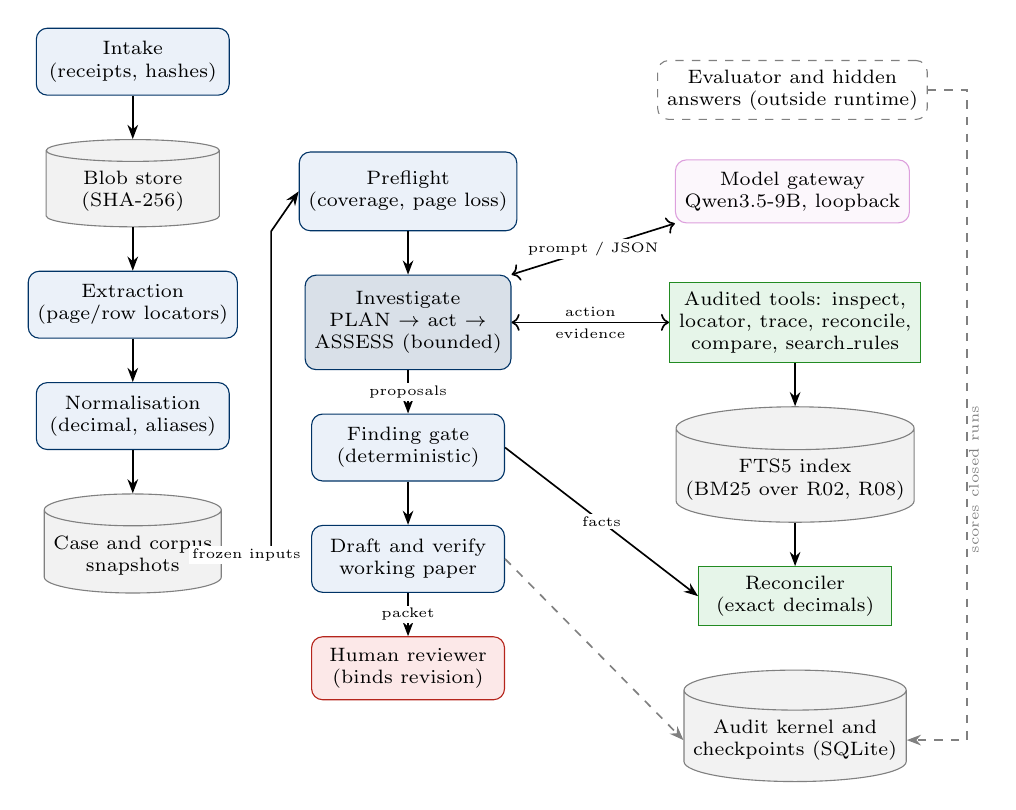
\begin{tikzpicture}[
  node distance=0.55cm and 0.5cm,
  comp/.style={draw=bmsblue,fill=guidebg,rounded corners,minimum width=2.45cm,minimum height=0.85cm,align=center,font=\scriptsize},
  tool/.style={draw=ForestGreen,fill=dobg,minimum width=2.45cm,minimum height=0.75cm,align=center,font=\scriptsize},
  store/.style={draw=gray,fill=gray!10,cylinder,shape border rotate=90,aspect=0.18,minimum width=2.2cm,minimum height=0.9cm,align=center,font=\scriptsize},
  human/.style={draw=BrickRed,fill=dontbg,rounded corners,minimum width=2.45cm,minimum height=0.8cm,align=center,font=\scriptsize},
  model/.style={draw=Plum,fill=Plum!8,rounded corners,minimum width=2.45cm,minimum height=0.8cm,align=center,font=\scriptsize},
  arr/.style={-{Stealth[length=1.8mm]},semithick},
  lab/.style={font=\tiny,fill=white,inner sep=1pt}]
% evidence column
\node[comp] (intake) {Intake\\(receipts, hashes)};
\node[store, below=of intake] (blob) {Blob store\\(SHA-256)};
\node[comp, below=of blob] (extract) {Extraction\\(page/row locators)};
\node[comp, below=of extract] (norm) {Normalisation\\(decimal, aliases)};
\node[store, below=of norm] (snap) {Case and corpus\\snapshots};
% workflow column
\node[comp, right=1.0cm of blob, minimum height=1.0cm] (pre) {Preflight\\(coverage, page loss)};
\node[comp, below=of pre, minimum height=1.2cm, fill=bmsblue!15] (inv) {Investigate\\PLAN $\rightarrow$ act $\rightarrow$\\ASSESS (bounded)};
\node[comp, below=of inv] (gate) {Finding gate\\(deterministic)};
\node[comp, below=of gate] (draft) {Draft and verify\\working paper};
\node[human, below=of draft] (review) {Human reviewer\\(binds revision)};
% tools column
\node[model, right=2.0cm of pre] (model) {Model gateway\\Qwen3.5-9B, loopback};
\node[tool, right=2.0cm of inv] (tools) {Audited tools: inspect,\\locator, trace, reconcile,\\compare, search\_rules};
\node[store, below=of tools] (fts) {FTS5 index\\(BM25 over R02, R08)};
\node[tool, below=of fts] (recon) {Reconciler\\(exact decimals)};
\node[store, below=of recon] (audit) {Audit kernel and\\checkpoints (SQLite)};
% evaluator
\node[draw=gray,dashed,rounded corners,align=center,font=\scriptsize,minimum width=2.45cm,above=0.5cm of model] (oracle) {Evaluator and hidden\\answers (outside runtime)};
% arrows
\draw[arr] (intake) -- (blob);
\draw[arr] (blob) -- (extract);
\draw[arr] (extract) -- (norm);
\draw[arr] (norm) -- (snap);
\draw[arr] (snap.east) -| node[lab,pos=0.25]{frozen inputs} ([xshift=-0.35cm]pre.south west) -- (pre.west);
\draw[arr] (pre) -- (inv);
\draw[arr] (inv) -- node[lab]{proposals} (gate);
\draw[arr] (gate) -- (draft);
\draw[arr] (draft) -- node[lab]{packet} (review);
\draw[arr,<->] (inv.north east) -- node[lab]{prompt / JSON} (model.south west);
\draw[arr,<->] (inv) -- node[lab,above=1pt]{action} node[lab,below=1pt]{evidence} (tools);
\draw[arr] (tools) -- (fts);
\draw[arr] (fts) -- (recon);
\draw[arr] (gate.east) -- node[lab]{facts} (recon.west);
\draw[arr,dashed,gray] (draft.east) -- (audit.west);
\draw[arr,dashed,gray] (oracle.east) -- ++(0.5,0) |- (audit.east);
\node[font=\tiny,gray,rotate=90] at ([xshift=0.75cm]fts.east) {scores closed runs};
\end{tikzpicture}
}
\end{frame}

\begin{frame}{The bounded investigation loop}
\begin{itemize}
\item LangGraph state graph: \textbf{preflight} $\rightarrow$ \textbf{investigate} $\rightarrow$
\textbf{draft} $\rightarrow$ \textbf{verify}, checkpointed in SQLite with compare-and-swap versions.
\item Each turn: \textsc{plan} proposes \emph{one} audited tool call (or stops with a reason);
the tool runs on the frozen snapshot; \textsc{assess} returns a verdict and resolve / continue /
abstain. Resolve requires \emph{supports}.
\item Six tools: inspect evidence, locator lookup, certificate trace, reconciliation, return
comparison, rule search (BM25 over the Rules and the CPCB FAQ, graded).
\item Bounds: 12 model calls, 600\,s, 32{,}768 tokens per call; repeated actions refused; invalid
output retried once, then deterministic evidence only.
\item Model: Qwen3.5-9B Q8\_0 on llama.cpp \texttt{b12033}, local, loopback only.
\end{itemize}
\end{frame}

\begin{frame}{Agentic concepts, with evidence}
\scriptsize
\begin{tabularx}{\linewidth}{@{}l c X@{}}
\toprule
\textbf{Concept} & & \textbf{Evidence} \\ \midrule
Tool use & \checkmark & six audited tools; every call recorded before dispatch \\
Agentic RAG & \checkmark & graded rule search; MG2 Retriever grades results and must re-query \\
Planning and reasoning & \checkmark & \textsc{plan}/\textsc{assess} loop; fixed (V1) vs adaptive (V2) \\
Observability & \checkmark & per-trial ledger, result records, audit-chain check \\
Evaluation & \checkmark & deterministic scorer, hidden answers, controls, bootstrap CIs \\
Multi-agent (bonus) & \checkmark & Retriever + Classifier, pre-registered, measured \\
Human in the loop, guardrails & \checkmark & finding gate; review bound to the report revision \\
Durable workflow & \checkmark & checkpoints and resume; queue resumes from ledgers \\
Experimentation & \checkmark & MG1 chain, MG2 experiment, one held-out run \\
Memory & partial & within a run only, by design (no leakage between cases) \\
\bottomrule
\end{tabularx}
\end{frame}

\begin{frame}{How it was evaluated}
\begin{itemize}
\item \textbf{48 synthetic dossiers} (\texttt{pilot-0.1}), sixteen fault families F01--F16, one per
family per split plus combinations; grouped splits, similarity checks.
\item \textbf{Splits:} tuning-16 (decisions), checking-8 (looked at once), held-out 24 (sealed, run
once). \textbf{Ablated arena}: tuning-16 with every deterministic family check off.
\item \textbf{Primary metric:} supported case success: exact buckets, exactly the expected finding
families, required scopes withheld, no forbidden action.
\item \textbf{Controls in every session:} V0 (no model) and SC (scripted controller). If a model arm
cannot beat SC, the model adds nothing measurable.
\item Hidden answers never enter the runtime; one Docker container per trial on the PC.
\end{itemize}
\end{frame}

\begin{frame}{MG1: the single agent}
\begin{itemize}
\item Prompt tuning plateaued: v7 succeeded on 69 of 128 tuning trials; the model contributed 3
findings.
\item Tracing the failures showed deterministic causes, so the \emph{engine} was fixed: family
checks and a contradiction gate took v7 to 30, then 32 of 32.
\item \textbf{But the controls matched it}, and the model's share of findings was 0.
\item With every family check off: V1, V2 and SC all 0 of 21 findings; a thinking prompt found 1
with false claims and regressed to 26 of 32 with the rules on.
\end{itemize}
\vspace{0.4em}
\begin{alertblock}{Reading}
The gains came from the deterministic engine. The model never read document text.
\end{alertblock}
\end{frame}

\begin{frame}{MG2: two agents, pre-registered}
\centering
\resizebox{0.95\linewidth}{!}{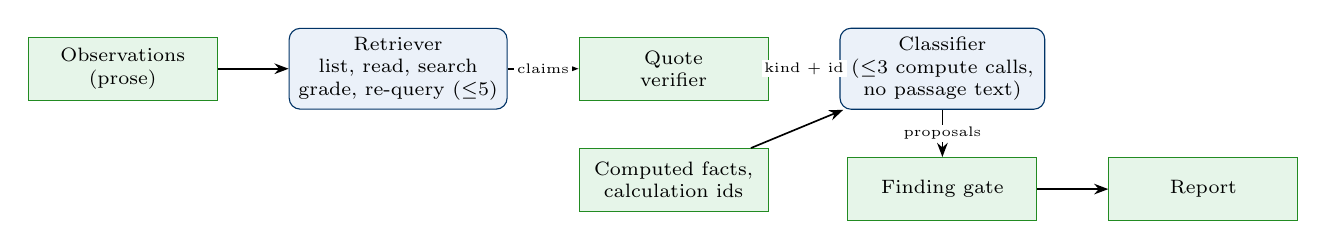
\begin{tikzpicture}[
  node distance=0.6cm and 0.9cm,
  comp/.style={draw=bmsblue,fill=guidebg,rounded corners,minimum width=2.6cm,minimum height=0.9cm,align=center,font=\scriptsize},
  det/.style={draw=ForestGreen,fill=dobg,minimum width=2.4cm,minimum height=0.8cm,align=center,font=\scriptsize},
  arr/.style={-{Stealth[length=1.8mm]},semithick},
  lab/.style={font=\tiny,fill=white,inner sep=1pt}]
\node[det] (obs) {Observations\\(prose)};
\node[comp, right=of obs] (ret) {Retriever\\list, read, search\\grade, re-query ($\le$5)};
\node[det, right=of ret] (ver) {Quote\\verifier};
\node[comp, right=of ver] (cls) {Classifier\\($\le$3 compute calls,\\no passage text)};
\node[det, below=of cls] (gate) {Finding gate};
\node[det, below=of ver] (facts) {Computed facts,\\calculation ids};
\node[det, right=of gate] (rep) {Report};
\draw[arr] (obs) -- (ret);
\draw[arr] (ret) -- node[lab]{claims} (ver);
\draw[arr] (ver) -- node[lab]{kind + id} (cls);
\draw[arr] (facts) -- (cls);
\draw[arr] (cls) -- node[lab]{proposals} (gate);
\draw[arr] (gate) -- (rep);
\end{tikzpicture}
}
\vspace{0.5em}
\begin{itemize}\small
\item \textbf{Hypothesis:} a Retriever that reads and grades text, plus a Classifier over verified
claims and computed facts, recovers judgement faults in the ablated arena without adding false
findings when the rules are on.
\item Arms M2 (both), M1 (Retriever + lookup), M2-nr (Classifier alone) against S1 (v7) and SC;
prompts v1--v3 declared in advance; selection rule fixed before the first run.
\item Ran on free Kaggle T4 GPUs as a separate series while the PC was down: 18 sessions, 1{,}008
trials, scored on the laptop.
\end{itemize}
\end{frame}

\begin{frame}{MG2 result: cost and benefit per arm}
\centering
\vspace{0.3em}
\resizebox{0.68\linewidth}{!}{\begin{tikzpicture}
\pgfplotstableread[col sep=comma]{generated/mg2-plot.csv}\mgtwo
\begin{axis}[ybar, bar width=7pt, width=\linewidth, height=6.2cm,
  ymin=0, ylabel={Findings (32 trials per arm)},
  xtick=data, xticklabels from table={\mgtwo}{label},
  x tick label style={rotate=35,anchor=east,font=\scriptsize},
  legend style={at={(0.5,1.03)},anchor=south,font=\scriptsize,draw=none},
  legend columns=2,
  nodes near coords, nodes near coords style={font=\tiny},
  axis lines*=left, ymajorgrids, grid style={gray!25}, enlarge x limits=0.07]
\addplot[fill=BrickRed!70,draw=BrickRed] table[x expr=\coordindex, y=rules_on_fp]{\mgtwo};
\addplot[fill=ForestGreen!60,draw=ForestGreen] table[x expr=\coordindex, y=ablated_tp]{\mgtwo};
\legend{{Accepted false positives (rules on)},{True positives (ablated)}}
\end{axis}
\end{tikzpicture}
}
\vspace{0.4em}

\begin{block}{Reading}\small No arm both recovers faults with the rules off and stays clean with them on.\end{block}
\end{frame}

\begin{frame}{MG2 result: the rules-on gate}
\slidetable{generated/mg2-rules-on.tex}
\end{frame}

\begin{frame}{Held-out run (24 sealed dossiers, once)}
\noindent{\small\color{inkgray} Declared before it ran (log entry 15): V1 vs V2 with v7 is the primary comparison;
V0, SC and the Classifier alone (v3) are descriptive.\par}
\vspace{-0.2em}
\HeldOutTable
\vspace{0.2em}
\begin{columns}[T]
\column{0.48\textwidth}
\begin{block}{Result}\footnotesize V1 and V2 tie with both controls at the ceiling; the engine generalises.\end{block}
\column{0.48\textwidth}
\begin{block}{What the model added}\footnotesize V2 needs 2.4 model calls against 6.1; accepted model findings: none.\end{block}
\end{columns}
\end{frame}

\begin{frame}{Decision and what we learned}
\begin{itemize}
\item \textbf{No multi-agent arm passed the gate.} Every Retriever arm accepted 25--38 false findings
in 32 trials, mostly F05 (wrong entity alias) and F14 (out-of-scope regime), whatever the prompt.
\item The Classifier alone was nearly clean only because the gate rejected almost everything it
proposed.
\item Prompt iteration stopped after three versions; the remaining budget went to one honest
held-out run, where every loop and control succeeded on all 24 unseen cases.
\item At this model size, the value is in the deterministic tools, the gate and human review. The
agent loop's demonstrated property is that it is \emph{bounded, traceable and safe to fail}.
\end{itemize}
\end{frame}

\begin{frame}{Limitations and responsible use}
\begin{columns}[T]
\column{0.5\textwidth}
\textbf{Limitations}
\begin{itemize}\small
\item Synthetic dossiers from one generator, built by the same team that built the system
\item Small sets; wide intervals
\item One 9B model only
\item T4 runs used process-level isolation
\item Why the gate accepts F05/F14 claims is not yet analysed
\end{itemize}
\column{0.5\textwidth}
\textbf{Responsible use}
\begin{itemize}\small
\item Advisory working paper only: no filing, trading or compliance verdict
\item Every finding cites evidence and calculations
\item A person reviews; the decision binds the exact revision
\item Local inference; no real producer data
\end{itemize}
\end{columns}
\end{frame}

\begin{frame}{Conclusion and future work}
\begin{itemize}
\item Built: an audited evidence pipeline, a bounded LangGraph agent with a deterministic gate and
human review, a 48-dossier benchmark with an isolated evaluator, and an unattended trial harness
for a GPU PC or a free cloud T4.
\item Measured: honest negative result for the model, positive for the design around it.
\item Next: analyse and close the gate's F05/F14 gap; rerun MG2 with a larger model; an
independently authored dossier set; more sources; held-out rerun with container isolation.
\end{itemize}
\vspace{0.8em}
\centering\small
Repository: \url{https://github.com/R-V-Abhishek/ReCycleGuard}\\[0.3em]
Report: \texttt{docs/report/report.pdf}
\end{frame}

\end{document}
